\section{Arquitectura del Sistema}
El componente central se organiza en capas de presentación, servicios de negocio, persistencia e integración. La presentación comprende los frontoffices, el backoffice y la API REST utilizada por los clientes. Los servicios de negocio concentran las validaciones y los controles de acceso a las operaciones, mientras que la persistencia permite almacenar y consultar la información del sistema. La integración con Usuario gub.uy, la PDI y los nodos de balanzas se realiza mediante adaptadores que separan la comunicación con estos sistemas de la lógica de negocio. La Figura \ref{fig:vista-logica} presenta la arquitectura general del sistema.

\begin{figure}
\centering
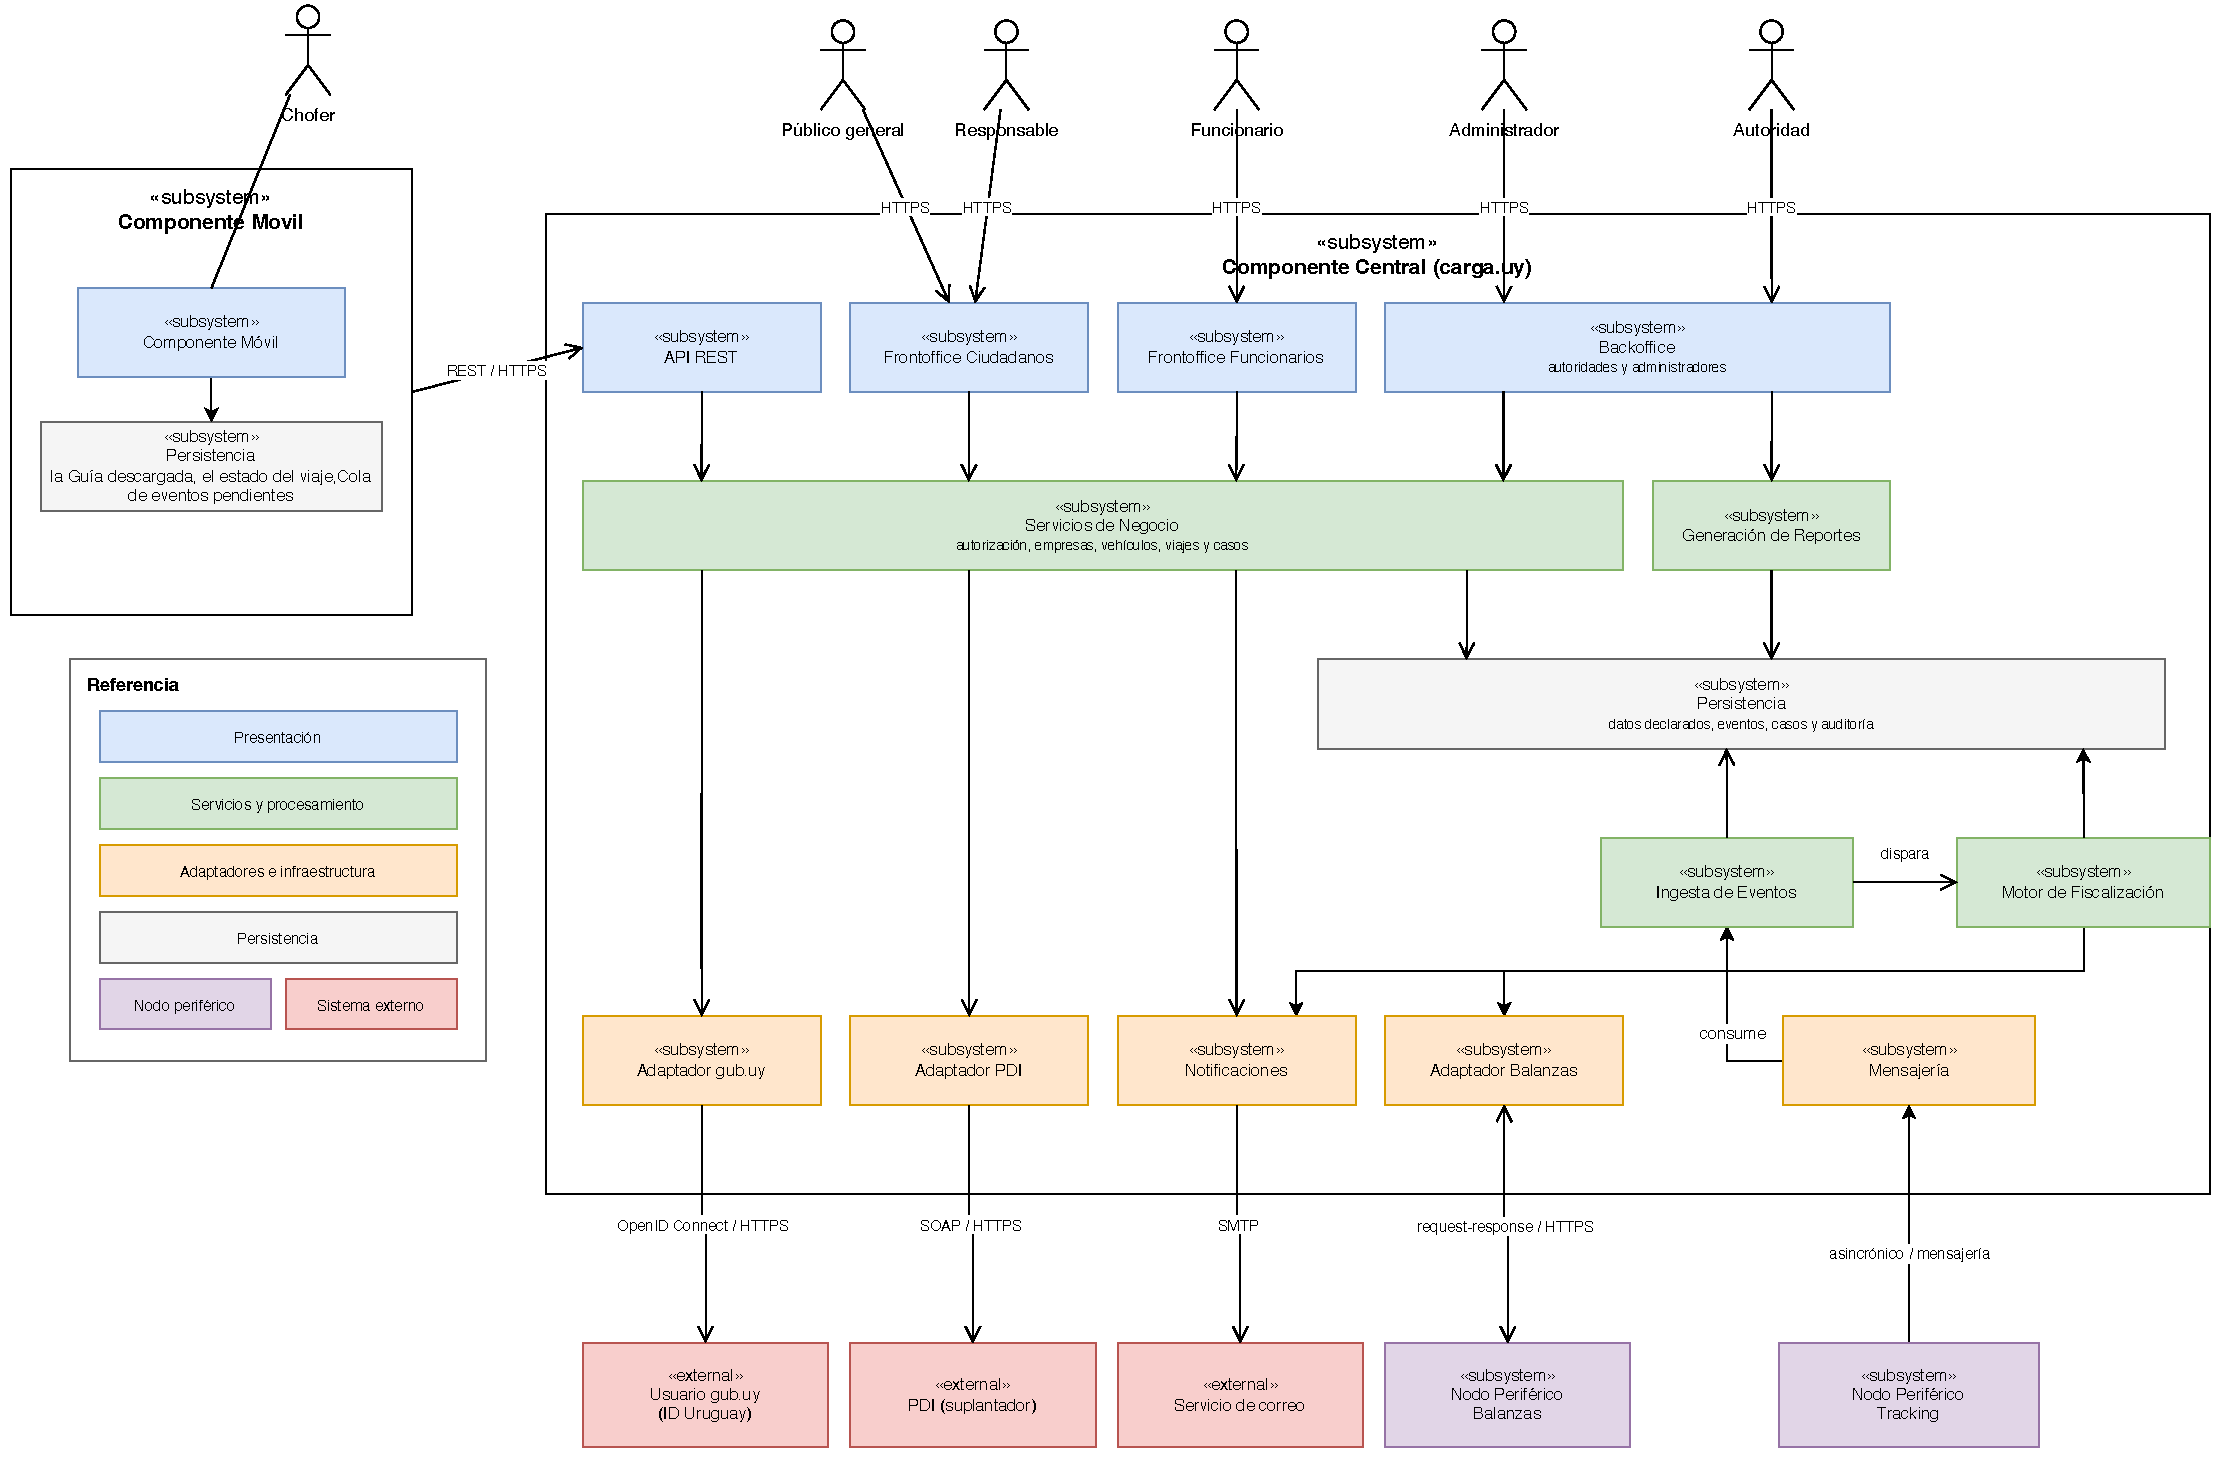
\includegraphics[width=\textwidth]{figuras/vista-logica.pdf}
\caption{Arquitectura general del sistema}
\label{fig:vista-logica}
\end{figure}

La recepción de las posiciones de tracking sigue un camino asíncrono: los nodos de tracking publican en un broker de mensajería que se ejecuta separado del servidor de aplicaciones, y el central las consume y las almacena en una base de datos documental, separada de la base relacional.
